\chapter{Software Development Model}
We identify our project as a software development task. To deliver a high quality software product in time, we have to study different development process models, and adopt an appropriate one. The software development model is an abstract process of how software is developed. As software engineering evolves, many software development models have been introduced. Despite of their differences, basically all these models involve the process of requirement analysis, architecture design, implementation, testing etc.

\section{Waterfall Model}
The waterfall model is a preliminary software development model. It breaks down the software development process into linear sequential phases. Each phase only depends on the output of the previous step. The developers have to work step by step, and there is no way to turn back.

\begin{figure}[htbp]
\centering
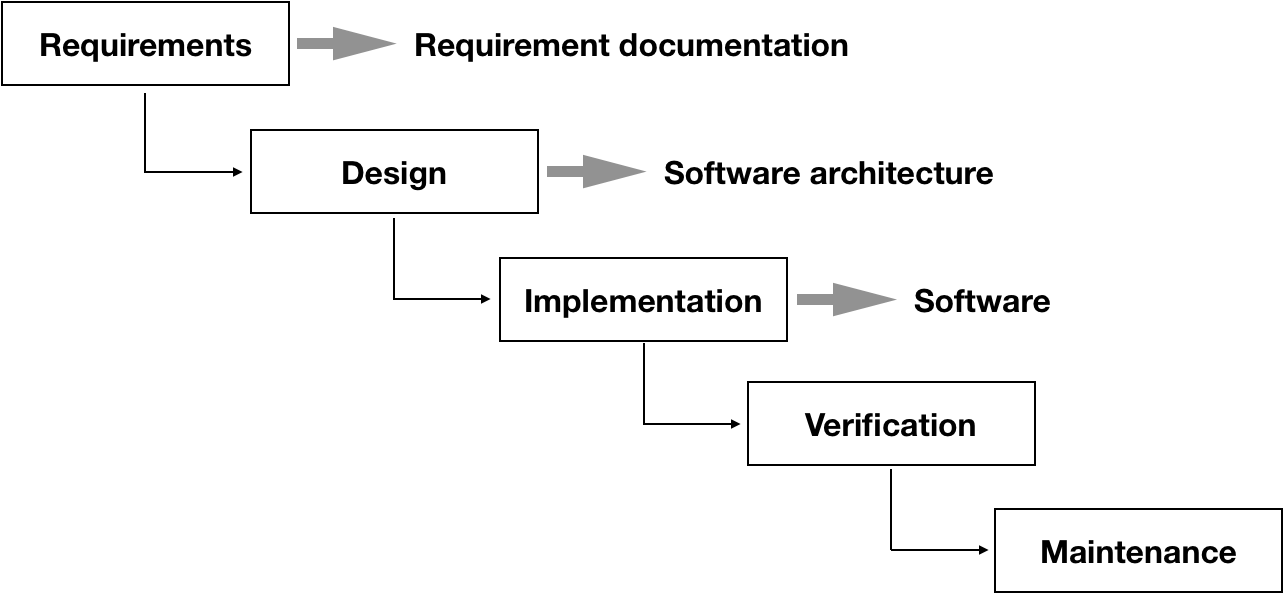
\includegraphics[width = \textwidth]{WaterfallModel}
\caption{Waterfall Model\label{fig:Waterfall Model}}
\end{figure}

The first step is requirement analysis. The developers use different methods to abstract user requirements, and make the system specifications. Requirement analysis is not as easy as it seems to be. There are many practical issues. In many cases, the developers do not have good access to users, making it difficult to analyze users' requirements. In fact, even the users themselves might not really know what they want. In some cases, due to lack of software engineering practice, users or clients might raise unrealistic requirements. When the user requirements are available, the developers have to make the system specifications, aka system requirements, which is a more detailed description of the software system. Finally, the output is a requirement documentation either in natural language or formulated language.

With the requirement documentation available, the developers have to design the software architecture. The design process is crucial in that the software architecture is difficult and costly to change in the future steps. A bad architecture can lead to poor testability, maintainability and quality. It also makes implementation more difficult.

When the architecture design is complete, we then implement the software. Then, we test the software and verify whether all requirements are satisfied. Finally, we deploy the software and maintain it in everyday use.

The waterfall model breaks down the software development process in a highly structured way. It pays attention to the early stages of the software development process, which tends to be neglected by many developers. According to studies, time spent at the early stages can lead to a great cost reduction in the later stages. A major drawback is inflexibility. The waterfall development process does not provide any way to adapt to changes in requirements. Also, there is no way to look back and make changes on the previous steps.

\section{V-Model}
The V-model is an extension of the waterfall model. It breaks down the development process into the project definition and the test and integration phases. Each development phase has an associated testing phase.

\begin{figure}[htbp]
\centering
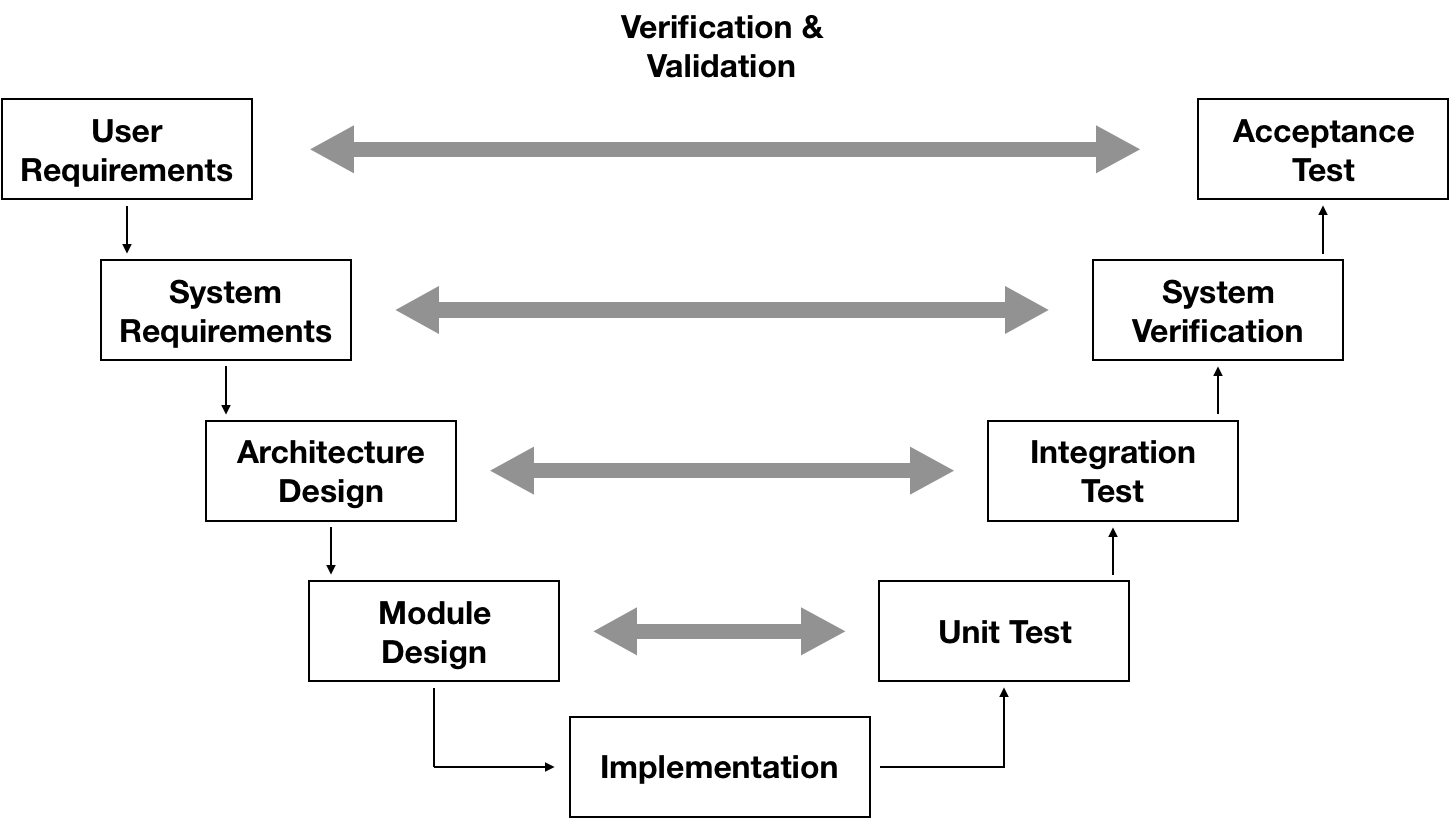
\includegraphics[width = \textwidth]{VModel}
\caption{V Model\label{fig:V Model}}
\end{figure}

The V-model places great importance on testing. However, it received similar criticisms as the waterfall model. The process is rigid and unable to well respond to change.

\section{Iterative Model}
To tackle problems with the waterfall model and the V-model and to introduce more flexibility, the iterative model was proposed. The idea is to repeat the whole development process and develop the software iteratively. After each iteration, the software is delivered to the users for evaluation and temporary use. Then, the developer works with the users and update the requirements. After that, the developer repeats the design, implementation and testing phases, and deliver an updated software to the users. Developers repeat this process until the users are satisfied, and then make the final deployable version.

\begin{figure}[htbp]
\centering
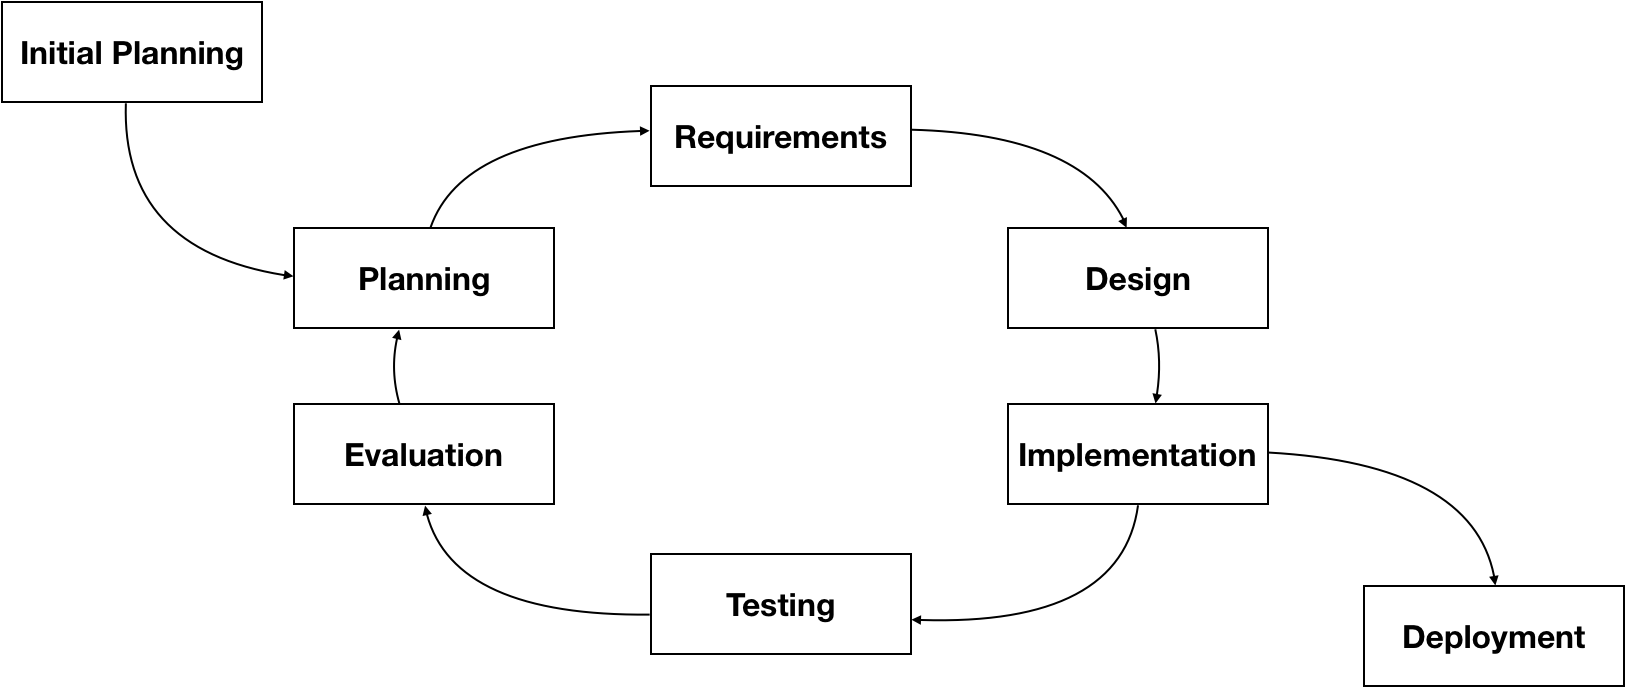
\includegraphics[width = \textwidth]{IterativeModel}
\caption{Iterative Model\label{fig:Iterative Model}}
\end{figure}

The iterative model differs to the waterfall model in many important ways. In the waterfall model, requirements, software design and code are fixed once they are finished. Users do not participate in the development process once requirements are fixed. The software is delivered only when the whole development process is complete. Finally, the waterfall model is only suitable for large projects. The iterative model, however, assumes everything is variable in the first place. After every iteration, users are involved in evaluation of the software. The software is developed incrementally, and can be delivered at early iterations. The iterative model is especially suitable for small projects, however, it can also benefit large projects.

\section{Prototype Model}
The waterfall model assumes requirements can be completely abstracted at the early stage of software development, and remain unchanged afterwards. In practice, however, initial requirements might not be complete and they can change over time. By building prototypes, the software developer can review the prototypes with users so as to update the requirements. In this way, users are involved early in the project and provide valuable feedback to the software developers. Prototyping is also a technique to verify whether the designed technical specifications are fulfilled. Based on existing prototypes, current implementation can be improved and prototypes evolve into the stereotype. Additionally, prototyping is also a good way for developers to get an initial idea of the project and estimate timelines of the project.

\begin{figure}[htbp]
\centering
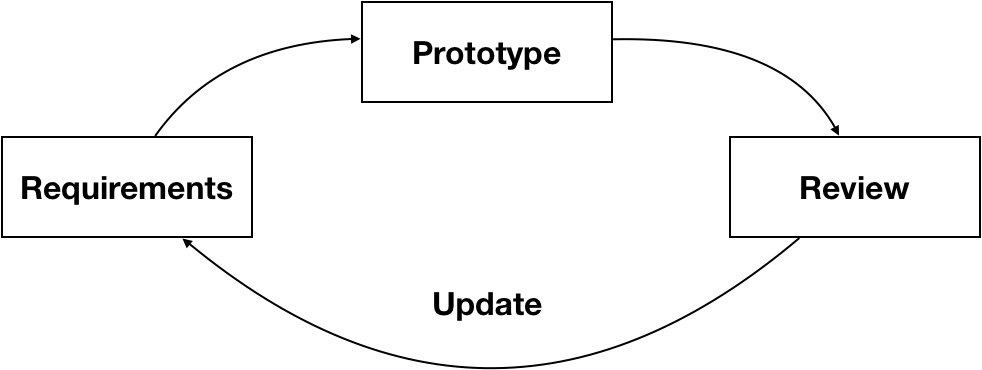
\includegraphics[width = \textwidth]{PrototypeModel}
\caption{Prototype Model\label{fig:Prototype Model}}
\end{figure}

In the field of software engineering, rapid prototyping is especially good for designing the user interface. It is not easy to know what the UI should exactly look like without building one. The developers first write preliminary requirements and a draft of the UI. Then, a prototype is built against the requirements. The prototype is reviewed by the users, and if necessary, the requirements are updated and the prototype is revised. Finally, the requirements are fixed.

Rapid prototyping is not concerned about implementation of complete functionalities, but only the some certain aspects like UI. Also, prototypes are made for review, and are thrown away afterwards. Sometimes rapid prototyping is also referred to as throwaway prototyping.

\section{Conclusion}
We investigated different classical software development models. Recent years, agile development and its variations have become increasingly popular. It emphasizes adaptive planning, face-to-face communication, incremental development and rapid delivery, adaptation to change, and collaboration between the development teams and users etc. It is a brand new development philosophy compared to the classical development models.

In our software development practice, we did not mechanically adopt a certain development model. To better understand the project, make the final version of the requirements and design the UI, we did rapid prototyping. In the following stages, we adopted an iterative and incremental strategy. We set up a weekly meeting to discuss the newly implemented functionality and the current development status. After the first version was complete, we delivered a beta version to the users. According to user feedbacks, we removed errors and made minor changes to the software. And finally, we made a product version and delivered it to the user.

In the whole development process, users actively participated. We responded to user feedbacks rapidly and adapted very well to changes in requirements. A scientific development process ensured that the software product was satisfactory, high quality, and delivered timely. 